(by Nourhan Omar)

\p
Three possible competitors were found for Posefix, and while they are not based in Europe, 
the products are sold online and could easily be delivered to customers in Germany, whether in the form of software or a physical device.

Below is the summary of the competitor's analysis:

\begin{table}[ht]
    \centering
    \begin{tabular}{|p{3cm}|p{3cm}|p{3cm}|p{3cm}|}
        \hline
        \textbf{Competitor} & \textbf{Zen} & \textbf{Posture AI} & \textbf{Upright} \\
        \hline
        Type & Software & Software & Physical Device \\
        \hline
        Device needed & Camera/Bluetooth headphones & Sensor/smart t-shirt & Sensor \\
        \hline
        Finances & Raised \$3.5M & 2 investors, still in beta phase & \$2.4M revenue/year, Acquired for \$31M \\
        \hline
        Target Customers & Consumers (B2C), Companies (B2B), Insurance Companies (B2B) & Consumers (B2C) & Consumers (B2C), Companies (B2B) \\
        \hline
        Pricing & Subscription-based model, \$9.99 - \$24.99 per year for consumers & One-time purchase: \$149 & One-time purchase: \$59.95-\$94.99 \\
        \hline
        Place & Online & Online & Online \\
        \hline
        Promotion & Online articles/social media & Online articles/website & Website/ articles/ social media \\
        \hline
        Skills & Cheap, easy access, bad UI & Expensive, had not fully launched, based in Seoul, Requires wearable (inconvenient) & Inconvenient wearable, good price, big market share, Android app store downloads \\
        \hline
    \end{tabular}
\end{table}    

\section{Zen}

\begin{figure}[H]
    \centering
    
\includegraphics[width=0.5\textwidth]{zen.png}
    \caption{Zen logo}
    \label{fig:zen}
\end{figure}

Zen is our main competitor as it has a very similar product to ours and is targeting similar customer groups as well. Zen is a software that detects your posture through the webcam if it's a desktop application or through the air pods if it's an iPhone application.  It was founded in October 2020 and is based in California in the United States \cite{zen_crunchbase}. It has raised $3.5$ million in 2021 from multiple investors including Y combinator\cite{posturehealth_ycombinator} and Valor Equity partners \cite{zen_techcrunch}. According to their LinkedIn\cite{posturehealth_linkedin} profile, they have tens of thousands of users. 

Zen has a \$9.99 yearly subscription if it's the mobile version and \$24.99 if it's the desktop version. It targets consumers, companies as well as medical institutions such as hospitals and insurance companies. It advertises through paid online articles and paid partnerships with influencers on social media, but the ads are mainly focused on the mobile application.

The good thing about Zen is that it's easily accessible on the phone as it can get downloaded from the Apple store and is cheap compared to other competitors. However, it takes a little digging to reach the desktop app, and the UI is non-intuitive making it hard to use. Additionally, it is mainly targeting customers in the US especially the companies and medical institutions.

\section{Posture AI}
\begin{figure}[H]
    \centering
    
\includegraphics[width=0.5\textwidth]{posture_ai.png}
    \caption{Posture AI logo}
    \label{fig:posture_ai}
\end{figure}

\begin{figure}[H]
    \centering
    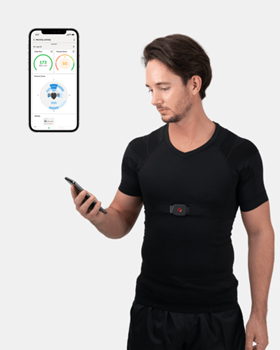
\includegraphics[width=0.5\textwidth]{wearable_ai.png}
    \caption{smart t-shirt}
    \label{fig:wearable_ai}
\end{figure}
Even though Posture AI launched 2 years ago and has 2 offices in Seoul \cite{postureai_linkedin} but the product is still in beta testing. It consists of a wearable t-shirt with a sensor that gets connected to a mobile application. The product is a one-time purchase at \$149 and could be ordered online through their website \cite{myposture}. The company mainly targets consumers and has 2 investors but they are not publicly known \cite{postureai_pitchbook}. The Android mobile app only has 50+ downloads. 

The product promises to improve posture through the “functional” shirt with an ergonomic design and the sensor that tracks your posture and provides real-time feedback yet the device does not seem practical as it requires wearing the shirt all the time which is unrealistic. Additionally, due to the high price of the product, the consumer won't be able to buy multiples to switch between.

\section{Upright}

\begin{figure}[H]
    \centering
    
\includegraphics[width=0.5\textwidth]{upright_logo.png}
    \caption{Upright logo}
    \label{fig:upright_logo}
\end{figure}

Upright has been on the market since 2014 \cite{uprightpose} and has received hype on social media during COVID-19 when people started working from home and focusing on their posture.
Upright is a physical device that sticks to the back of the consumer and is connected to a mobile application that has over 50 thousand downloads in the Android app store.
It buzzes whenever the consumer slouches to instantly warn them to adjust their posture.
The product is promoted through their website and social media and earns \$2.4 million per year through selling their product \cite{upright_growjo} ranging from \$59.95 to \$79.95.
The price differs whether the consumer buys the device with 2 or 3 sensors and whether they buy the accessories set or the standalone device.
The company was acquired by Dario Health for \$31 million in 2021 \cite{dariohealth_acquisition}.

\begin{figure}[H]
    \centering
    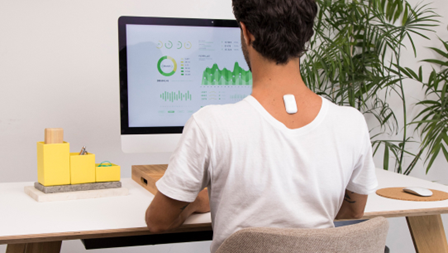
\includegraphics[width=0.5\textwidth]{upright_device.png}
    \caption{Upright Go 2 device}
    \label{fig:upright_device}
\end{figure}

The company is based in Israel but targets end consumers across the globe through its online website and selling through third-party such as Amazon. The cons of this product are that the consumer has to keep wearing the product and that it only targets one point in the body.

\section{Competitive Strategy}

Our competitive strategy is a differentiation focus strategy where we aim for our product to be a technological and user experience leader by providing the latest technologies to accurately detect the consumer's posture without the need for any external device or sensor other than the camera. 

Additionally, we would focus on providing a better user experience by focusing on consumer privacy as well as providing leaderboard scores and competition badges to encourage consumers to keep using the application. We would also focus our strategy on the German market, especially German workplaces as none of our competitors are focusing on the German market yet.